\subsection{The target class cannot be duplicate with any imported class from another package.}

If a class is imported from another package, we have to pre-check that the target class meant to be rename refactored does not match with the imported class. This is because the compiler will not be able to distinguish between the imported class and the existing class. 

\begin{figure}[th]
\centering
\begin{minipage}[t]{0.6\linewidth}
\begin{lstlisting}[language=java, basicstyle=\scriptsize\ttfamily,frame=single]
package beforevisitor;
class A{
    
}	
class Test{

}

package aftervisitor;
import beforevisitor.Test;
class A{

}
class B{

} 

\end{lstlisting}
\tiny{(a) Before Rename Refactoring Class B}
\end{minipage}
\hfill

\begin{minipage}[t]{0.6\linewidth}
\begin{lstlisting}[language=java, basicstyle=\scriptsize\ttfamily,frame=single]
package beforevisitor;
class A{
    
}	
class Test{

}

package aftervisitor;
import beforevisitor.Test;
class A{

}
class Test{

} 
\end{lstlisting}
\tiny{(b) After Rename Refactoring Class B to Test}
\end{minipage}
\caption{Precondition when importing a class}
\label{figure:fig2}
\end{figure}

In Fig. \ref{figure:fig2} (a), we see that class B is not a duplicate for class A and class B can be rename refactored to any other name instead of A as mentioned in section \ref{sec:precon1}. However, in Fig. \ref{figure:fig2} (b), when we try to rename refactor the class B to class Test, we get compile error \textit{"a compilation unit must not import and declare a type with the same name"}~\cite{EclipseWebPage}. 
This is because a class named Test is being imported from another package and on renaming the target class B to Class Test will have compilation error due to duplicate names. 

\begin{figure}[th]
\centering
\begin{minipage}[t]{0.75\linewidth}
\begin{lstlisting}[language=java, basicstyle=\scriptsize\ttfamily,frame=single]
package aftervisitor;
public class Visitor {
  public void print() {
      System.out.println("Hello");
  }
}

package beforevisitor;
import aftervisitor.Visitor;
class A {
    public static void main(String[] args) {
        Visitor v = new Visitor();
        v.print();
    }
}

\end{lstlisting}
\tiny{(a) Before Rename Refactoring Class A}
\end{minipage}
\hfill

\begin{minipage}[t]{0.75\linewidth}
\begin{lstlisting}[language=java, basicstyle=\scriptsize\ttfamily,frame=single]
package aftervisitor;
public class Visitor {
  public void print() {
      System.out.println("Hello");
  }
}

package beforevisitor;
import aftervisitor.Visitor;
class Visitor {
    public static void main(String[] args) {
        Visitor v = new Visitor();
        v.print();
    }
}
\end{lstlisting}
\tiny{(b) After Rename Refactoring Class A to Visitor}
\end{minipage}
\caption{Class already defined in Compilation Unit}
\label{figure:error}
\end{figure}


\begin{figure}[H]
\centerline{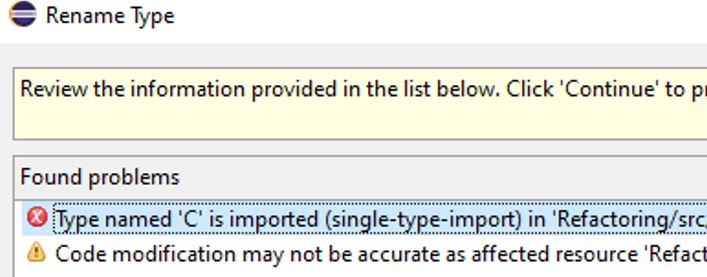
\includegraphics[width=85mm,scale=0.5]{CUE.jpg}}
\caption{The Compilation Unit Error}
\label{figure:pic}
\end{figure}

Another example where rename refactoring requires a pre-check if the target name is not already defined in the compilation unit is shown below . In Fig. \ref{figure:error} (a), on executing the output generated is \textit{Hello}. However, after rename refactoring class A to Visitor as shown in Fig. \ref{figure:error} (b), we get compile error as shown in Fig. \ref{figure:pic}.
\\Therefore, it is essential to pre-check that the target class should not have duplicate name with any of imported class after rename refactoring class. 




